\chapter{Inferring the Localization of White-Matter Tracts using Diffusion Driven Label Fusion}

\section{Overview}
In the previous chapters we studied the structural organization of the brain,
and saw that it is highly related to function. Some white matter pathologies,
such as tumors or traumatic brain injury, affect the white matter to the point
were it's impossible to use tractography. Therefore, we cannot tell which
tracts are affected. Given the relationship between brain and function, it's
important to determinate which tracts were affected in order to prevent
which function will be affected.
In this chapter, we introduce a way to infer the location of pathways, even
when it's not possible to use tractography to locate them. Our technique is
based on a methodology named label fusion. In particular, we show how to add
dMRI information to the label fusion in order to better estimate the location
of white matter pathways.

This work was presented as part of OHBM 2018~\cite{Guillermo2018}.

\section{Introduction}
Pathologies such as traumatic brain injuries, brain tumors or edemas disrupt
the structure of white matter, resulting in cognitive deficits. Depending on
the type and severity of the pathology, fiber bundles can be displaced,
infiltrated or directly interrupted~\cite{Schonberg2006, Huisman2009, Won2016}.
Inferring which pathways are affected, or surround the pathology is key for both
pre and post-treatment planning. With this knowledge, neurologists and
neurosurgeons can decide if a lesion should be treated more aggressively or 
conservatively~\cite{Huisman2009, McGirt2009}. Diffusion MRI allows to
non-invasively reconstruct white matter tracts by means of tractography. In
healthy brains, tractography is able to recover the major fiber bundles in the
brain~\cite{Catani2008}. However, in the presence of pathologies, tracking
through the white-matter becomes challenging.

Four types of patters can be identified in major tracts and diffusion
information affected by a brain pathologies~\cite{Pictorial2004} . The first
pattern consists of normal Fractional Anisotropy (FA)~\cite{Basser1996}, and
tract displacement~\cite{Pictorial2004}. In this case, a
bundle is displaced by the tumor, without interrupting it. The second pattern
is substantially decreased FA with no tract displacement, this could be
an edema or small tumor\cite{Schonberg2006, Huisman2009}.
The third pattern is substantially decreased FA with some lost of directionality,
for which tracking becomes hard~\cite{Schonberg2006, Pictorial2004}. Finally,
the fourth pattern consists of isotropic diffusion within the pathology,
which causes a disruption of the tracts~\cite{Pictorial2004}.
In this last case, it's possible to track until, and after the tumor, but not
within it.

The third and fourth patterns presented 
denote situations in which the tracking results in interrupted or erroneous
tracts. The incorrect shape of the resulting tracts, or its lack of continuity
makes hard to infer which pathways are directly affect by the pathology. In these
cases were it's not possible to use tractography, aggregating spatial information
from other subjects in order to infer the affected tracts could be a solution.
Assuming we defined major bundles in a group of healthy subjects, we could
register them to the brain of our patient and combine them using a label fusion
technique. Label fusion is a family of techniques which aim is to infer the
localization of a structure in a target subject, based on its
localization in a group of control subjects.

\begin{figure*}[t]
    \includegraphics[width=\textwidth,height=150px]{missing}
    \caption{Graphical explanation of the voting process}
    \label{fig:weighted_diffusion}
\end{figure*}

One well known label-fusion technique is Majority Voting~\cite{Xu1992}. Given a
voxel on a brain image, each subject is said to "vote" for a label. The resulting
voxel label will be that with the most votes. Majority Voting is simple to
implement and has been demonstrated to yield accurate segmentations~\cite{Asman2013}
in healthy subjects. However, this technique is blind both to registration problems
and anatomical variability between subjects. To overcome this, it has been propose
to weight the vote of each subject by how similar the subject looks to the
target~\cite{Sabuncu2010}. The underlying intuition is that the choosing of labels
should be driven by those subjects who resemble the most to the one being labeled.
The practical advantages of various strategies based on this idea have recently
been demonstrated by Artaechevarria et al.~\cite{Artaechevarria2009}.

Current label fusion techniques rely only on anatomical information, not taking 
into account the structure of white matter. In the case of white matter pathways,
the presence of a path constrains the diffusion of water particles, which can be
measured by dMRI. Therefore, adding diffusion information to the fusion algorithm
could help to better delineate fiber bundles. In this work, we introduce a new 
label fusion technique that, taking advantage of dMRI, weights the vote of each
subject based on how the voted pathway is supported by the test subject's diffusion
data. This is, if the diffusion data of the test subject is consistent with the
direction of the voted pathway, the vote has a higher weight. Our technique also
allows to work with crossing tracts, by modeling multiple labels per voxel.

We validate our technique in 9 subjects of the Human Connectome Project (HCP).
For each subject, we infer the location of 4 left hemisphere tracts using
whole-brain tractography and an implementation of the white matter query language
(WMQL). We use this results as ground truth to compare against inferring the
tracts from using the other 8 subjects with our proposed technique and Majority
Voting. Our results show that our proposed techniques achieves a higher level
of precision. This is, our technique is able to give a more trustable labeling,
incurring in the trade-off of labeling less voxels. We also show that our technique
is able to label around simulated brain lesions.

This work is organized as follows: In the Methods section we make an introduction
to label fusion techniques and present how to extend them using diffusion
information. In the Experiments and Results section we present our results 
both on synthetic and on HCP data. We then discuss our results and position
ourselves with respect to the state of the art in the Discussion section. 
Finally, in the last section we provide our conclusions.



\section{Methods}
\label{sec:methods}

\subsection{Majority Voting}
Let $labels = \{l_i\}, \forall_i l_i \in N$ be the set of labels representing
tracts and grey matter structures in one hemisphere. Let ${L_s}, s \in S$
represent the labeling of a set of subjects $S$, where each 
$L_s \in labels^{v\times v}$ is a 3D volume representing the labeling of a
specific subject. Majority Voting~\cite{Rohlfing2004} infers the label of
each voxel $x$ in the test subject ($L(x)$) by computing:

\begin{equation}
\label{eq:mvoting}
\begin{aligned}
    \hat L(x) = \argmax_{l \in labels} \sum_{s\in S} p(L(x) = l | L_s(x)),\\
    \text{where} \\
    p(L(x) = l | L_s(x)) =
    \begin{cases}
        1,& \text{if } L_s(x) = l \\
        0,& \text{otherwise}
    \end{cases}
\end{aligned}
\end{equation}

In this case, it's said that each subject in the training set votes for a label
per voxel, and the label with the most amount of votes is assigned to the target
voxel.

\subsection{Diffusion Based Voting}
Our label fusion technique takes advantage of dMRI to weight the vote of each
subject. The vote for a specific label gets a higher weight if it's supported
by the diffusion data of the subject being labeled. In this section, we first
start explaining the concept of Orientation Density Function of diffusion in
dMRI and tract directionality. Then, we present how to use these concepts to
compute the weights of each vote.

\subsubsection{Fiber Orientation Density Function from dMRI Data.}
By fitting the diffusion information into a Constrained Spherical Deconvolution (CSD)
model, it's possible to estimate a fiber orientation density function\cite{Tournier2004} (fODF). 
The fiber ODF $F_x(\theta, \phi)$ represents the estimated fraction of fibers
within the voxel $x$ that are aligned along the direction $(\theta, \phi)$,
expressed in spherical coordinates.

\subsubsection{Fiber Orientation Density Function from Tractography.}
A tract can be described as a set of streamlines, were a streamline is a
discretrized 3-dimensional curve. Assuming that a streamline doesn't have sharp
turns, we can estimate its directionality within a voxel by looking at its
entry and exit points (Fig. \ref{fig:weighted_diffusion} A). Repeating this for each streamline
on a tract, we obtain a set of directional vectors, representing the directionality
of the tract within the voxel. A fiber ODF can be estimated from this set of
vectors by means of directional statistics. In this work, we use an
Angular Central Gaussian Distribution~\cite{Mardia1999} (ACGD). The ACGD models
antipodal symmetric directional data. It has a close form to estimate its
parameters, making it easier to use than other directional distributions on the
sphere~\cite{Mardia1999}.
    
% Since we also want to estimate directionality from tracts, we introduce the concept of acgd
\subsubsection{Label Fusion Weighted by Diffusion}
Majority Voting (Eq. \ref{eq:mvoting}) decides the label of a voxel based on
how many subjects 'vote' for it. Given that we are interested in inferring
white-matter paths, we introduce a weight to each vote driven by diffusion
information:

%We want to introduce a weight to these votes, taking into account how well the
%tract can explain the underlying Diffusion data of our test subject. In
%particular, we want to the Orientation Distribution Function (ODF) of our
%test subject's diffusion. This is, we want to profit of the fact that we know
%how the water particles are moving in its brain, following the underlying tracts.
%As explained in section X, in a given voxel, we can compute the main
%directionality of the tract $l$ of the train subject $s$ and the ODF of our
%test subject's diffusion. To see if the tract are aligned with the
%directionality of the voted tract we proposed the following model:

\begin{equation}
\label{eq:mvoting_weighted}
\hat L(x) = \argmax_{l \in labels} \sum_{s\in S} p(L(x) = l ; L_s(x)) p(D(x) ; D_{sl}(x)).
\end{equation}

In our segmentation scheme, the term $p(L(x) = l ; L_s(x))$ is modeled in the same
way as in the voting scheme (eq. \ref{eq:mvoting}). Our second term,
$p(D(x) | D_{sl}(x))$ express the probability of seeing the diffusion of our
target subject ($D(x)$) on voxel $x$, given that the tract $l$ is passing through
it with a shape as in subject $s$ ($D_{sl}(x)$). Intuitively, if subject $s$ votes
for the tract $l$, the weight represents how much they tract $l$ in voxel $x$
assembles the diffusion of the target subject in the same voxel. We model this
second term as:

\begin{equation}
\label{eq:inner_odf}
\begin{aligned}
    p(D(x) ; D_{sl}(x)) = 
    \begin{cases}
        <F(x), F_{sl}(x)>,& \text{if } L_s(x) = l,\\
                        & \text{and } l \neq 0 \\
        <F(x), U>,& \text{if } L_s(x) = 0 \\
        0,& \text{otherwise}
    \end{cases} \\
    \text{where} \\
    <F(x),F(x)> = 1,\\ < F_{sl}(x), F_{sl}(x)>=1.
\end{aligned}
\end{equation}

In our model, $F(x)$ is the fiber ODF on voxel $x$ estimated from the diffusion
of the target by means of CSD. It's normalized in such a way that the inner
product with itself results in 1. $F_{sl}(x)$ is the fiber ODF of the tract $l$
registered from subject $s$, estimated by means of ACGD. $U$ is a uniformly
distributed fiber ODF, this is the diffusion assumed for either the label 
no-tract, representing the background or a gray matter structure.
By computing the inner product between ODFs, we can estimate how much they look
alike. This allow us to weight the votes of each subject, while accounting for
the white-matter structure of both the voting subjects and the target.
\begin{figure*}[t]
    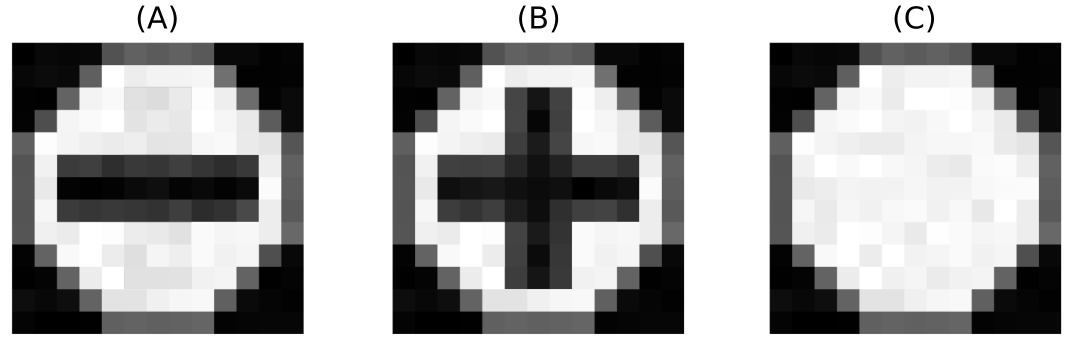
\includegraphics[height=150px]{7.multiatlas/img/phantoms.png}
    \caption{Phantoms created to test how our technique weights the votes.
             (A) Only one tract in the white matter (B) Two tracts crossing. (C) No tracts, free diffusion.}
    \label{fig:pha_exp_1}
\end{figure*}

\section{Experiments and Results}
In section \ref{sec:methods} we presented how to add diffusion information to
Majority Voting (Eq. \ref{eq:mvoting_weighted}). This allow us to weight each
vote by how much the diffusion of the target supports it. Now, we present
experiments both in phantoms and subjects from the Human Connectome 
Project (HCP). We start by assessing that the computed weights correctly reflect
the diffusion information in dwi phantoms. Then, we proceed to infer the localization
of white-matter pathways in subjects of the HCP, and compare them with their
truth shape. Finally, we simulate lesions in the white-matter and test the
performance of our method.

\subsection{Data and Preprocessing}
We created three types of diffusion weighted image phantoms using Phantomas~\cite{Caruyer2014}.
The first phantom possess only one tract, traveling from one side to the other of the
image horizontally (Fig. \ref{fig:pha_exp_1} A). The second possess two crossing tracts,
forming a 90 degrees angle between them (Fig. \ref{fig:pha_exp_1} B). The last, has no
fibers, and represents isotropic diffusion (Fig. \ref{fig:pha_exp_1} C). From
each one of them, we generated 31 DWIs. All the DWIs were generated using a
Signal to Noise Ratio of 20, and a resolution of $1mm$ per voxel. The final
images are 3-dimensional matrices, with 10 voxels in each dimension. Having
such small images, allows us to test how our label fusion technique behaves
on a controlled environment.

To test our technique in more realistic scenarios, we randomly selected 9 subjects
from the HCP500 dataset from the Human Connectome Project. For each subject,
we computed whole-brain tractography using each voxel in the white-matter as
a seed and simulating 8 particles per seed~\cite{Garyfallidis2014}. We extracted
the main tracts from the left hemisphere tractogram (13 tracts in total) using
the implementation of the white-matter query language (WMQL)~\cite{Wassermann2016}.
For each subject we computed registrations to the rest using as reference their
T1w images~\cite{Jenkinson2012}. Using the resulting warp transformations, we
registered the tracts between every pair of subjects.

For both the phantom DWIs and the HCP subjects, we estimated their fiber ODFs
using the implementation of CSD in Dipy~\cite{Garyfallidis2014}. The ODFs were
discretrize on a sphere with $n=100$ vertices. A uniform distribution over the sphere
was created by assigning to each vertex the value $\sqrt(n)/n$, making $<U, U> = 1$.


\begin{figure*}[t]
    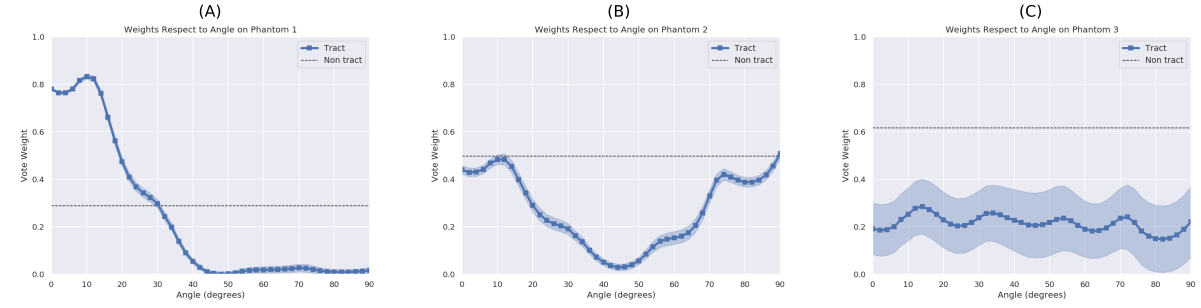
\includegraphics[width=\textwidth]{7.multiatlas/img/weights.png}
    \caption{We started with an horizontal tract and start rotating it. We computed
             the weight a subject would get when voting for the tract. 
             (A) Weights in phantom A (B) Weights in phantom B (C) in C.}
    \label{fig:pha_exp_1}
\end{figure*} 

\subsection{Assessing the Correctness of Voting Weights in Synthetic Data}
In order to study how the tract's directionality influences its vote weight,
we started by recreating the tracts present in the first phantom (Fig. \ref{fig:pha_exp_1} A).
For this, we took one of the 31 DWIs, and computed 1000 streamlines by means of 
probabilistic tracking from the voxels in which the tract passes. In the DWIs
generated from the first phantom, this tract is the one that should generate the
highest weight. At the same time, any change in its directionality, should decrease
the weight. To test this, we computed the weights obtained by the estimated tract
and planar rotations of it around the central voxel in the remaining 30 DWIs.
Figure \ref{fig:pha_exp_1} A shows the obtained weights on the first phantom.
Effectively, the weight starts to rapidly decrease as the angle increments and 
the directionality of the tract moves away from that of the diffusion.
Figure \ref{fig:pha_exp_1} B shows the weights obtained when repeating the 
experiment using 30 DWIs of the second phantom (Fig. \ref{fig:pha_exp_1} B),
which have a crossing of fibers in the central voxel. In this case, the weight
is higher when the tract is aligned to one of the crossing fibers (at 0 degrees
or 90 degress), while rapidly decaying in between them. Finally,
(Fig. \ref{fig:pha_exp_1} C) shows the weights when using 30 DWIs with
isotropic diffusion (Fig. \ref{fig:pha_exp_1} C). In this case, the weight
is always low, driven by the discrepancy between the directionality of the tract
and the free diffusion present in the DWIs.

To assess that the proposed model is not overweighting tracts, we also computed
the weight that a 'non-tract' label would receive in each of the phantoms. As
explained in section \ref{sec:methods}, equation \ref{eq:inner_odf}, when a
subject is voting for a non-tract label, a uniform fiber ODF is compared against
the diffusion ODF. The three subfigures composing figure \ref{fig:pha_exp_1}
also show the weight obtained in the central voxel when a subject is voting for
the label 'no-tract'. In figure \ref{fig:pha_exp_1} A, we can see that the
weight of 'no-tract' is low, specially when compared with the high weight
of the correctly aligned tracts (low angle rotations). This is driven by the
highly directional underlying diffusion data of the phantom. 
Figure \ref{fig:pha_exp_1} B shows that the weight of a 'no-tract' vote is
similar to that of an aligned tract. In this case, the underlying crossing
diffusion matches better with the uniform ODF. Finally, figure \ref{fig:pha_exp_1} C
shows always a higher weight for the 'non-tract' than for any tract, consistent
with the isotropic diffusion of our third phantom.

%Since our method is based on a weighted majority voting, the final result of
%the parcellation will depend not only on the weights, but also on the amount of
%subjects voting for each structure.
%Having the ability to compute the weights received by a structure allow us to
%examine what would happen in particular scenarios. Lets assume that only two types
%of subjects are voting, one type of subjects votes for a specific tract, and
%the other type of subjects votes for 'no tract'. The dotted lines in figure
%\ref{fig:pha_exp_1} show which proportion of subjects are needed to vote
%for the 'tract' in order for it to appear in the final segmentation. For
%example, in the phantom with one tract, the weight for the 'tract' with 0 degrees
%is such that only a 30\% of the subjects are needed to vote for it. Meanwhile,
%for tracts at 90 degrees, 70\% of the subjects are needed to vote for it. 
%In the phantom case when there's only isotropic DWI, we always need more than
%50\% of the subjects. These results show a good behaviour of our technique. 

\subsubsection{Inferring Tracts in Human Connectome Project Subjects}
To validate our technique in a more realistic but yet controlled scenario, we
inferred single tracts in the HCP subjects. We selected the following tracts to
work with: inferior part of the Superior Longitudinal Fasciculus (SLF1),
Inferior Longitudinal Fasciculus (ILF), middle part of the
Corpus Callosum (CC2), and External Capsule (EC). These four tracts provide
a fair diversity of directionality, shape, and position in the brain.

For each tract we performed a leave-one-out cross-validation. At each step, we
inferred the tract of one subject from the registered tracts of the others
using both Majority Voting and our technique. Using as 'ground truth' the
target's bundle computed by means of tractography and WMQL, we quantified the
performance of both techniques. In particular, we computed their confusion matrix.
A confusion matrix is a matrix $M \in \R^(2\times2)$, where each the entry $M_{ij}$
represents the number of times the label in the ground truth was i and the
technique labeled j. Finally, we computed the sensitivity, and precision on
each confusion matrix [cite]. Sensitivity measures the proportion of voxels
in the ground-truth tract that were 'discovered'. Precision measures the proportion
of voxels that were correctly labeled, over all the labeled voxels. Table 1 shows
the results obtained for each technique and tract. In all of the tracts, our
technique achieves a lower sensitivity than Majority Voting. This means that
we label a smaller portion of the ground-truth bundle. On the other hand,
our diffusion weighted label-fusion always achieve a higher precision. This
is, if we only look at the labels created by the techniques, our technique
has the highest proportion of correct ones. Another way to phrase it is, our
technique has a lower number of false positives.
Therefore, our technique is discovering less voxels, but those which are labeled
can be trusted more. Figure \ref{fig:labeling} shows a visual example of this.

\begin{figure*}[t]
    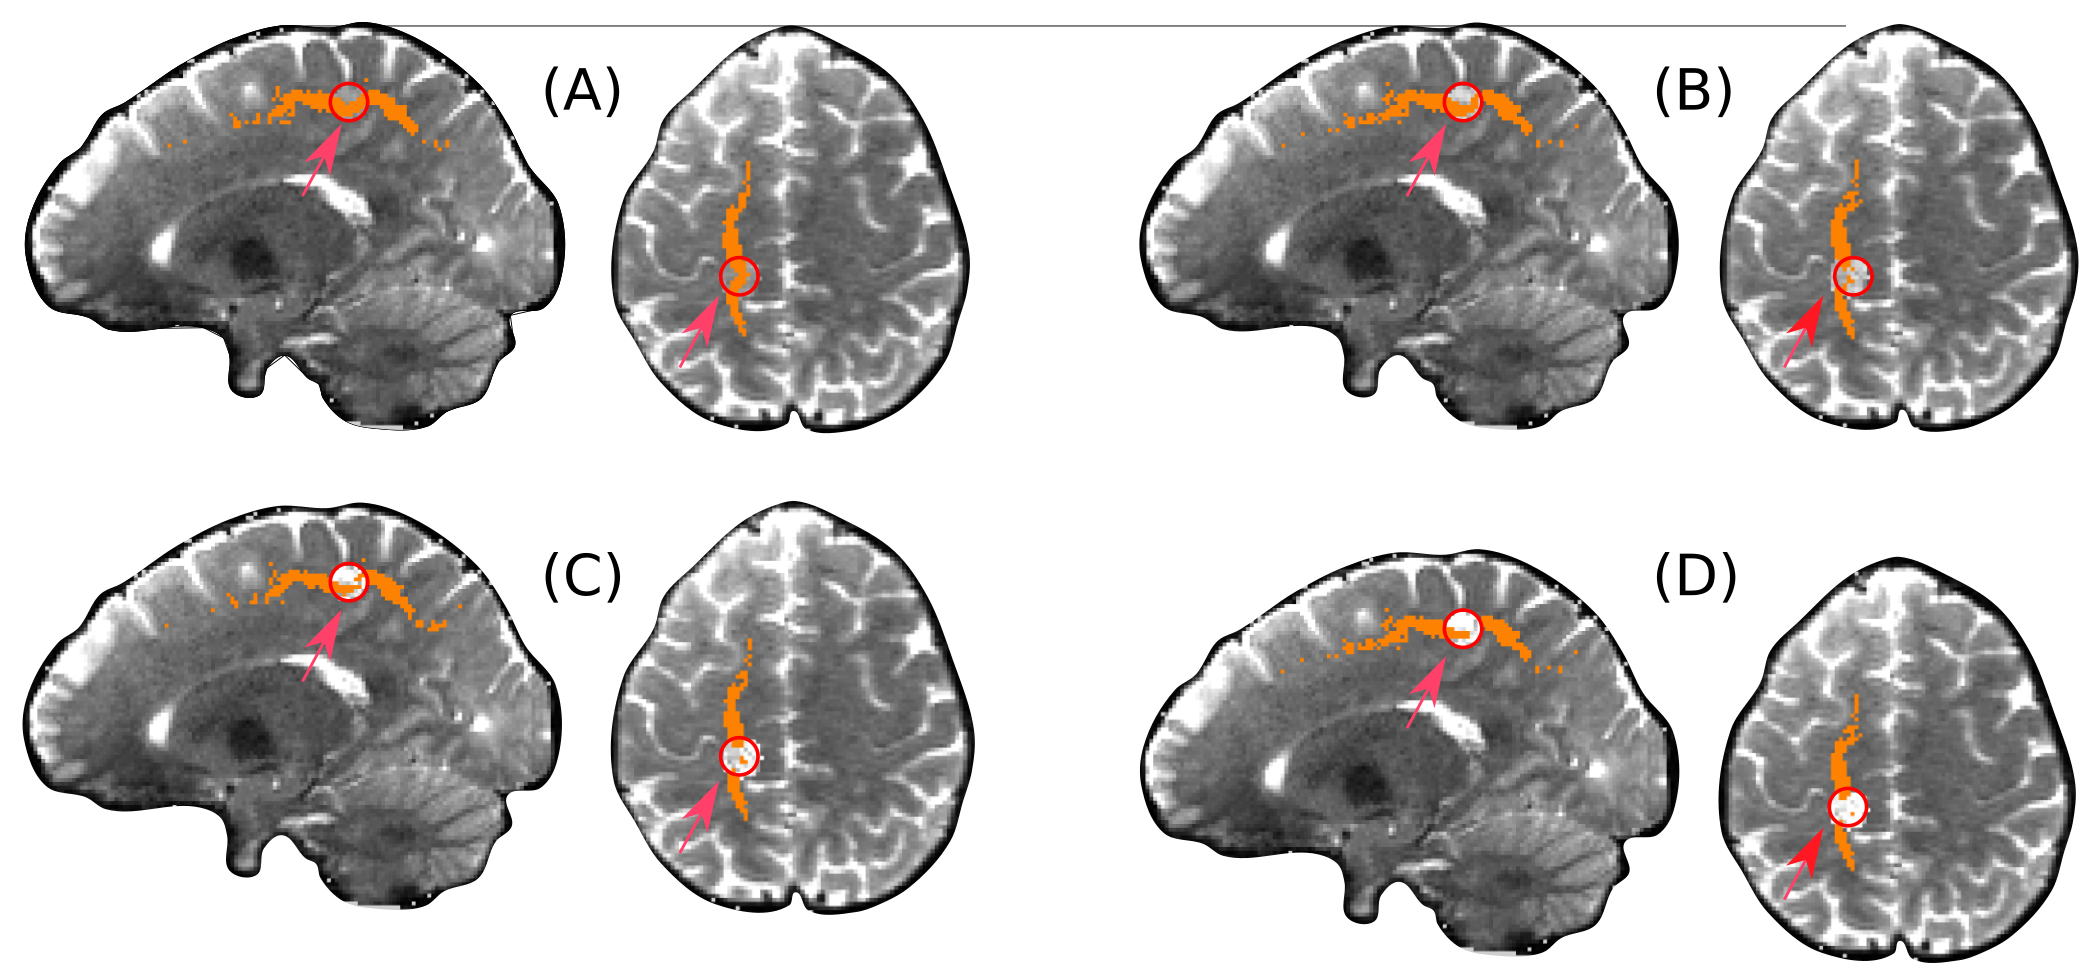
\includegraphics[width=\textwidth]{7.multiatlas/img/pathology.png}
    \caption{Test of tract retrieval when a lesion (red circle) is present.
             Lesions were simulated by mixing the signal with isotropic data,
             following eq. \ref{eq:mixing}. (A) $\alpha=0.2$
             (B) $\alpha=0.5$ (C) $\alpha=0.75$ (D) $\alpha=1$. Our technique
             labels less voxels as alpha increases.}
    \label{fig:labeling}
\end{figure*}

\subsubsection{Inferring Tracts in the Presence of Simulated Lesions}
To test how our technique behaves on an injured brain, we simulated
lesions at different degrees of severity in the white matter of one of our subjects.
Given that some brain lesions directly affect FA~\cite{Schonberg2006, Huisman2009},
we simulated lesions by adding isotropic signal to a set of voxels, therefore
lowering their FA. We targeted the SIF bundle, in order to compare how the labeling
changes. We did so by selecting a spherical region of $4mm$ where the SIF passes by, and mix
the diffusion signal there with signal from he ventricles. Since the ventricles
are regions filled with cerebrospinal fluid (CSF), their diffusion is approximately
isotropic. In particular, for each voxel $x$ in the lesioned region, we chose a
voxel $v$ in the ventricle and mix their signals ($S(\cdot)$) as follows:

\begin{equation}
    \label{eq:mixing}
S(x) = S(x)(1-\alpha) + S(v)\alpha, \alpha \in [0,1],
\end{equation}
where $\alpha$ manages the severity of the lesion. $\alpha=0$ represents healthy
tissue, and $alpha=1$ represents a total disruption of the white-matter,
resulting in pure isotropic diffusion. Figure \ref{fig:} shows that, at higher
alpha (lower FA), less voxels are labeled within the lesion. This is a
good behaviour, since by lowering the FA we make the diffusion more isotropic,
loosing the underlying tract. In particular, for $\alpha=1$, the diffusion
is completely isotropic, meaning that there's no tract, therefore, it's correct
to not label it. Since our technique still labels the surroundings of the
pathology, it allows to correctly identify the affected tract.

%WMQL stops detecting the ILF at... and our technique stops detecting it in the voxels at .... 

\subsection{Discussion}
In this work we presented a label-fusion techniques to infer white-matter
structures in the brain. In particular, we introduce diffusion weights to Majority
Voting~\cite{Xu1992}, a technique that has been demonstrated to yield accurate
segmentations~\cite{Asman2013} from few subjects. Being able to infer information
from few subjects is a major advantage,  to be able to ting is that it can be used with a low number of
registered subjects. The main advantage of our technique is
that it weights Majority Voting using diffusion information. In particular, our technique
weights the votes based on the similarity between the voted structure and the
diffusion of the target subject. By doing so, our technique does not rely only
on spatial features, as Majority Voting does.



Problems of registration.
We introduce a new way to take into account the diffusion information.
This makes a lot of sense, since we are trying to infer tracts, and the 
diffusion data is related to the underlying tracts.
We avoid registering diffusion, but we still have the white matter info.
In synthetic data, we show that our technique is much better than
majority voting, specially when the tracts align correctly with the
underlying diffusion. It also works like charm, when the tracts are completely
missaligned with the diffusion. In other cases, is as good as majority voting.
In real data, this is reflected, by showing that diffusion voting is more
conservative. WMM lessions.
Does this actually works? Registration is difficult around tumors.


The election of an uniform distribution comes from the fact that, in order to
be labeled, you should look closet to them than the free diffusion case.


\subsubsection{Our Technique Creates Weights Consistent With the Underlying
               Diffusion Data.}
In order to study how the tract's directionality influences its vote weight,
we created three different phantoms, and DWIs from them. Taking profit of 
these DWIs, we computed the weight of tracts with different directions. 
The weights obtained in figure \ref{fig:pha_exp_1} A show that, tracts
with a directionality similar to the underlying diffusion get higher votes.
But, the more we rotate the tract respect to the central voxel, the lower the
weight it obtains. In particular, after reaching an angle of 20 degrees, the
weight starts to drop rapidly, falling bellow the weight of the 'non-tract' label.
The Figure \ref{fig:pha_exp_1} B shows that the tracts aligned with one of the 
crossing fibers get weights similar to 'non-label'. In this case, if the tract
is roughly aligned with the underlying diffusion, then it will compete with
equal weights against the background. Finally, Figure \ref{fig:pha_exp_1} C
shows that, when there's no underlying white-matter structure in the DWI image,
then the label 'no-trac' is the one that receives the highest weight. These
results show that our technique is able to correctly weight each label based
on white-matter features, as diffusion directionality.

\subsubsection{Our Technique Incurred in a Trade-off Between the Amount of
               Labeled Voxels and Their Correctness.}
To test our technique in realistic data, we registered tracts between different
subjects of the HCP. Using these registered tracts, we inferred the position
of individual tracts in each subject. Table \ref{table:sensitivity} shows that
in each inferred tract, our technique achieved a lower sensitivity but a higher
precision. In fact, the precision, except for the External Capsule, is always
higher than 0.7. This means that our technique was able to discover less voxels,
but those who are labeled are mostly correct. Figure \ref{fig:labeling} shows
this in a visual way. Based on both the table and the figure, it's possible
to assess that Majority Voting is having a higher sensitivity just because
it's labeling more voxels. This is also what is causing it to have a precision
lower than 0.41 in all the tracts. Also, visually, our tracts are more spatially consistnt.


\subsubsection{Our Technique Behaves Correctly in the Presence of Pathologies}
We focused
in two types of pathologies: edema-like pathology, or tumor-like with no
deformation of the white-matter around it. As explained in the introduction, the
edema-like pathologies are characterized by a decreased FA. Meanwhile, the
tumor-like with no tract displacement are characterized by isotropic diffusion.
In order to simulate both lessons, we 


We are not taking into account mass effect



\subsection{Conclusions}
In this chapter we presented a labeling fusion technique that relies on dMRI
data to infer the localization of white-matter tracts. The results show that
our technique is more conservative than the voting rule, which is desired when
studying pathologies, at the cost of having more false negatives.


\begin{table*}[]
    \label{table:sensitivity}
\centering
    \caption{Sensitivity and precision of our proposed
             method (Weighted) and Majority Voting (Majority) when inferring single
             bundles in 9 subjects. The inferred bundles are: Superior Longitudinal
             Fasciculus (SLF), Inferior Longitudinal Fasciculus (ILF), Corpus
             Callosum (CC), and the External Capsule (EC).}
\label{my-label}
\begin{tabular}{|l||c|c||c|c||c|c||c|c|}
\hline
 & \multicolumn{2}{c||}{SLF} & \multicolumn{2}{c||}{ILF} & \multicolumn{2}{|c||}{CC} & \multicolumn{2}{|c|}{EC}\\ 
 \hline
            &  Weighted & Majority & Weighted & Majority & Weighted & Majority & Weighted & Majority \\
  \hline
Sensitivity & 0.19      & \bf{0.30}   & 0.33      & \bf{0.47}   & 0.53      & \bf{0.64}   & 0.06      & \bf{0.27} \\
  \hline
Precision   & \bf{0.70}      & 0.58   & \bf{0.74}      & 0.41   & \bf{0.91}      & 0.82   & \bf{0.42}      & 0.31 \\
\hline
\end{tabular}
\end{table*}

Figure 1. Outline of our technique. We extract the main white-matter tracts using WMQL, register them to the 'test' subject and then compute a voting rule weighted by diffusion information. For each voxel $x$ in the 'test' subject, we select the label $l$ that maximizes equation \ref{eq:argmax}, where S is the set of 'train' subjects, $t$ is the 'test' subject; $L_i(x)$ is the label of voxel $x$ for the subject $i$; $P$ are the principal directions of diffusion in the 'test' subject and $D_{sl}(x)$ are the directions of tract $l$ in the voxel $x$ of the 'train' subject $s$.

\chapterbib
